% !TeX program = pdflatex
% !TeX encoding = UTF-8
% !TeX spellcheck = es_ES

\documentclass[9pt, handout]{beamer}

%********************************************************************
% Packages
%********************************************************************

\usepackage[utf8]{inputenc}
\usepackage[T1]{fontenc}
\usepackage[english]{babel}
\usepackage[bottom, para]{footmisc}
\usepackage{amsmath,amssymb,amsthm}
\usepackage{graphicx}
\usepackage{hyperref}
\usepackage{listings}
\usepackage{perpage}
\usepackage{xcolor}
\usepackage{wrapfig}
\usepackage{ifthen}
\usepackage{scrextend} % add margin to answers
\usepackage{dashrule}

%********************************************************************
% Packages options
%********************************************************************

% geometry
\usepackage{geometry}
\geometry{
    a4paper,
    ignoremp,
    bindingoffset = 1cm, 
    textwidth     = 13.5cm,
    textheight    = 21.5cm,
    lmargin       = 1cm,
    rmargin		    = 3cm,
    tmargin       = 2cm,
    bmargin       = 3cm
}

% listings
\renewcommand{\lstlistingname}{Code}

\definecolor{lightgray}{rgb}{.9,.9,.9}
\definecolor{darkgray}{rgb}{.4,.4,.4}
\definecolor{purple}{rgb}{0.65, 0.12, 0.82}
\lstset{
  basicstyle=\small\sffamily,
  numbers=left,
  numberstyle=\tiny,
  numbersep=3pt,
  stepnumber=1,
  frame=tb,
  columns=fullflexible,
  backgroundcolor=\color{yellow!15},
  keywordstyle=\color{blue}\bfseries,
  ndkeywordstyle=\color{darkgray}\bfseries,
  identifierstyle=\color{black},
  commentstyle=\color{purple}\ttfamily,
  stringstyle=\color{red}\ttfamily,
  numberbychapter=false,
  showstringspaces=false,
  breaklines=true,
  captionpos=b, % put captions at the bottom 
}
%\lstset{
%  numbersep=5pt,
%  frame=trbl
%}

\definecolor{prismgreen}{rgb}{0.12, 0.48, 0.12}
\lstdefinelanguage{prism}{ % syntax highlight via font
  keywords={
    bool,C,ceil,const,ctmc,double,dtmc,endinit,endmodule,endrewards,endsystem,F,false,floor,formula,G,global,I,init,int,label,max,mdp,min,module,nondeterministic,P,Pmin,Pmax,prob,probabilistic,R,rate,rewards,Rmin,Rmax,S,stochastic,system,true,U,X
  }, 
  keywordstyle={\bfseries\color{black}}, 
  numberstyle=\tiny\color{black}, 
  comment=[l] {//}, morecomment=[s]{/*}{*/}, % single and multi-line 
  commentstyle= \color{prismgreen}, % dark green 
  tabsize=4, % tab treatment (going to be fixed in Prism)
  escapechar=@ % write LaTeX comments escaped by @ symbol 
} 

% perpage
\MakePerPage{footnote}

% hyperref
\definecolor{webgreen}{rgb}{0,.5,0}
\definecolor{webbrown}{rgb}{.6,0,0}
\definecolor{RoyalBlue}{cmyk}{1, 0.50, 0, 0}
\hypersetup{%
  %draft, % = no hyperlinking at all (useful in b/w printouts)
  colorlinks=true, linktocpage=true, pdfstartpage=3, pdfstartview=FitV,%
  % uncomment the following line if you want to have black links (e.g., for printing)
  % colorlinks=false, linktocpage=false, pdfstartpage=3, pdfstartview=FitV, pdfborder={0 0 0},%
  breaklinks=true, pdfpagemode=UseNone, pageanchor=true, pdfpagemode=UseOutlines,%
  plainpages=false, bookmarksnumbered, bookmarksopen=true, bookmarksopenlevel=1,%
  hypertexnames=true, pdfhighlight=/O,%nesting=true,%frenchlinks,%
  urlcolor=RoyalBlue, linkcolor=black, citecolor=webbrown, %pagecolor=RoyalBlue,%
  %urlcolor=Black, linkcolor=Black, citecolor=Black, %pagecolor=Black,%
}

% graphicx
\graphicspath{{img/}}

%********************************************************************
% New commands
%********************************************************************

\newcommand{\question}[1]{%
  \vspace{20pt}%
  \begin{wrapfigure}{l}{0.1\textwidth}%
    \vspace{-30pt}%
    \begin{center}%
      
\includegraphics[scale=1]{hand.jpg}%
    \end{center}%
    \vspace{-30pt}%
  \end{wrapfigure}%
  \noindent #1%
}%
\newcommand{\answer}[1]{%
  \vspace{5pt}\par\noindent
  \textbf{\underline{Answer:}}%
  \begin{addmargin}[1em]{1em}% 1em left, 2em right
    #1%
    \begin{flushright}%
      \qedsymbol%
    \end{flushright}%
  \end{addmargin}%
}%

\definecolor{light-gray}{gray}{0.95}
\newboolean{inlineCodeBackground}
\setboolean{inlineCodeBackground}{false}
\newcommand{\prism}[1]{%
  \ifthenelse{\boolean{inlineCodeBackground}}{%
    \colorbox{light-gray}{\lstinline[language=prism]{#1}}%
  }{%
    \lstinline[language=prism]{#1}%
  }%
}%
\newcommand{\bash}[1]{%
  \ifthenelse{\boolean{inlineCodeBackground}}{%
    \colorbox{light-gray}{\lstinline[language=bash]{#1}}%
  }{%
    \lstinline[language=bash]{#1}%
  }%
}%

\newcommand{\dashedrule}{%
  \noindent\hdashrule{\textwidth}{1pt}{1.5mm}%
}%


\title[AAL y modelos estocásticos]{Ambient Assisted Living y modelos estocásticos}
\author{\textbf{Tommaso Papini}}
\institute{
  STLab, Departamiento de la Ingenieria de la Informacíon, Universidad de Florencia, Italia,\\
  {tommaso.papini@unifi.it}
}
\date{
  29 de Mayo 2017\\
  {\small Departamento de Informática, Universidad de Jaén, España}
}

\begin{document}

  \begin{frame}
    \titlepage
    \begin{itemize}
      \item Ambient Assisted Living
      \item Modelos y datasets
      \item Análisis de entornos inteligentes
    \end{itemize}
  \end{frame}

  \begin{frame}{Overview}
    %\tiny
    \tableofcontents
  \end{frame}
  
  \section{Ambient Assisted Living}
    
    \begin{frame}{Ambient Assisted Living}
      El \textbf{Ambient Assisted Living} es un sector de investigación que tiene como objetivo ayudar a las personas que viven en \textit{entornos inteligentes} (es decir, dotados de sensores y actuadores) explotando a la tecnología de sensores y de procesamiento de datos.
      
      \begin{center}
        
\includegraphics[scale=1.8]{elderly_assi.jpg}
      \end{center}
    \end{frame}
    
    \subsection{Objetivos}
      \begin{frame}{Objetivos}
        \pause
        Un \textit{entorno inteligente} es un sistema \textbf{parcialmente observable}:
        \pause
        \begin{itemize}
          \item el estado efectivo del sistema resulta oculto;
          \pause
          \item solo se pueden observar eventos (\textit{observaciones}) emitidos por el sistema (por ej. la activación de un sensor).
        \end{itemize}
        
        \vspace{1em}
        \pause
        Principales análisis de interés:
        \pause
        \begin{itemize}
          \item \textbf{Diagnosis}: estimar cual es el estado efectivo actual del sistema a partir de las observaciones registradas.
          \pause
          \item \textbf{Predicción}: estimar cual será el estado efectivo del sistema después de una determinada cantidad de tiempo o la densidad de probabilidad de que un evento se verifique.
          \pause
          \item \textbf{Planificación de acciones}: elegir la acción optima y entre cuanto tiempo debe desarrollarse para evitar situaciones críticas.
        \end{itemize}
        
        \vspace{1em}
        \pause
        Análisis en linea:
        \pause
        \begin{itemize}
          \item intenta analizar un entorno inteligente \textit{mientras} está evolucionando.
        \end{itemize}
      \end{frame}
    
  \section{Modelos y datasets}
    \subsection{Modelos estocásticos}
      \begin{frame}{Modelos estocásticos}
        \pause
        Los \textit{modelos estocásticos} representan una aproximación de sistemas donde se modelan:
        \pause
        \begin{itemize}
          \item la evolución del estado del sistema;
          \pause
          \item parámetros estocásticos que definen como el sistema pasa de un estado al otro.
        \end{itemize}
        \pause
        \visible<5->{
          \begin{center}
            \colorbox{white}{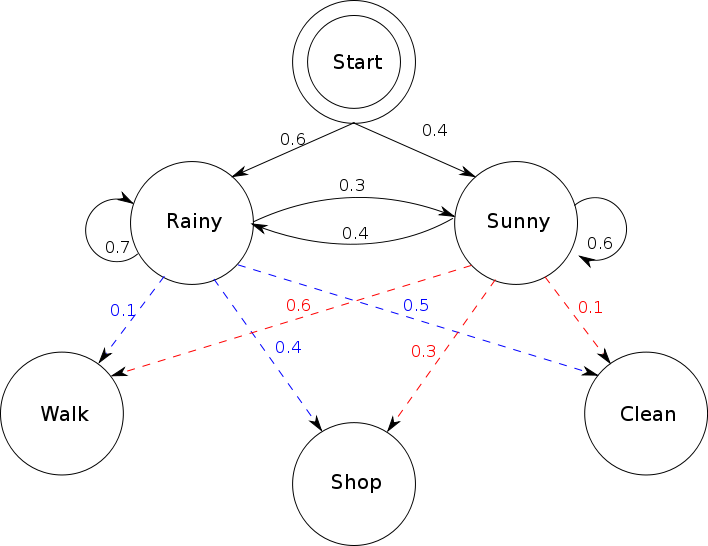
\includegraphics[scale=0.28]{708px-HMMGraph.png}}
          \end{center}
        }
      \end{frame}
    
    \subsection{Datasets anotados}
      \begin{frame}{Datasets anotados}
        \pause
        Un \textit{dataset anotado} es un dataset donde hay:
        \pause
        \begin{itemize}
          \item los eventos registrados y cuando han pasado (marca temporal);
          \pause
          \item anotaciones manuales de la evolución del estado efectivo del sistema (con intervalos temporales por cada estado).
        \end{itemize}
        
        \pause
        \vspace{1em}
        \visible<5->{
          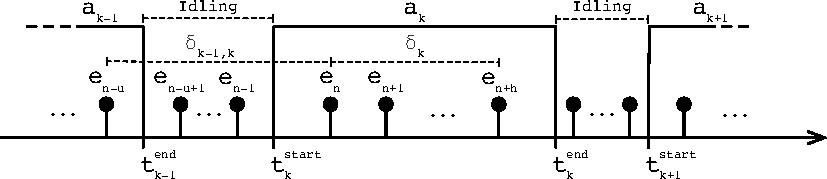
\includegraphics[scale=0.8]{activity_event_formulation.pdf}
        }
      \end{frame}
      
      \begin{frame}{Datasets anotados}{van Kasteren}
        Un ejemplo clásico de dataset anotado para AAL es el dataset de \textit{van Kasteren}\footnote{\url{https://sites.google.com/site/tim0306/datasets}}\footnote{Van Kasteren, T., Noulas, A., Englebienne, G. and Kröse, B., 2008, September. Accurate activity recognition in a home setting. In Proceedings of the 10th international conference on Ubiquitous computing (pp. 1-9). ACM.}
        
        \pause
        \visible<2->{
          \begin{center}
            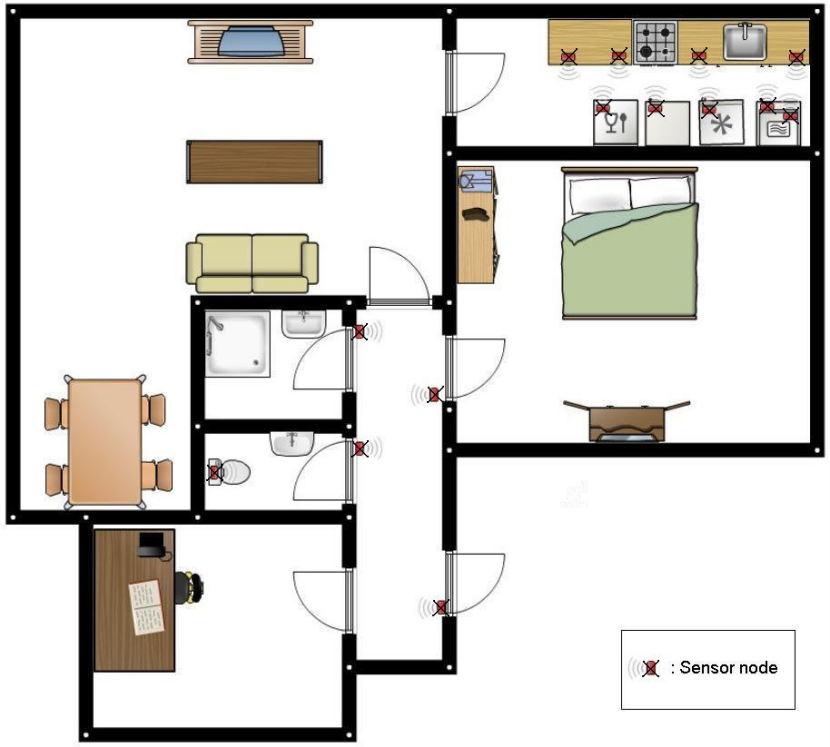
\includegraphics[scale=0.18]{SmartHome.png}
          \end{center}
        }
      \end{frame}
    
    \subsection{Process mining}
      \begin{frame}{Process mining}{De datasets anotados a modelos estocásticos}
        \pause
        Con el término \textbf{process mining} se indica un conjunto de técnicas para construir un modelo estocástico de un sistema parcialmente observable a partir de un dataset anotado de este mismo sistema.
        
        \pause
        \vspace{1em}
        El process mining está compuesto por dos técnicas principales:
        \pause
        \begin{itemize}
          \item \textbf{Process elicitation}: construye un modelo discreto (es decir, sin informaciones sobre la permanencia en los estados del sistema) a partir de los eventos y actividades anotados en el dataset.
          \pause
          \item \textbf{Process ehnancement}: añade una visión temporal continua a un modelo discreto introduciendo parámetros estocásticos que describen como el sistema evoluciona a lo largo del tiempo utilizando medidas estadísticas sacadas por el dataset.
        \end{itemize}
      \end{frame}
    
  \section{Análisis de entornos inteligentes}
  
    \begin{frame}{Análisis de entornos inteligentes}{Esquema general}
      \vspace{-1em}
      \begin{center}
        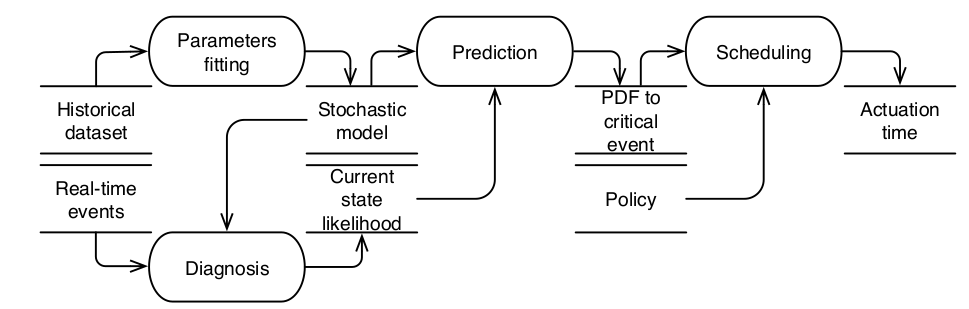
\includegraphics[scale=0.34]{architecture.png}
      \end{center}
      
      \pause
      \begin{itemize}
        \item \textbf{Process mining}: de dataset anotado a modelo estocásticos.
        \pause
        \item \textbf{Diagnosis}: de eventos efectivos a probabilidad del estado corriente (sobre un determinado modelo estocástico).
        \pause
        \item \textbf{Predicción}: de probabilidad del estado corriente a probabilidad de que ocurra un evento crítico.
        \pause
        \item \textbf{Planificación}: de probabilidad de que ocurra un evento crítico a tiempo de planificación de una reacción (con una determinada política de reacción).
      \end{itemize}
    \end{frame}
  
    \subsection{Diagnosis}
      \begin{frame}{Diagnosis}
      	\begin{center}
      		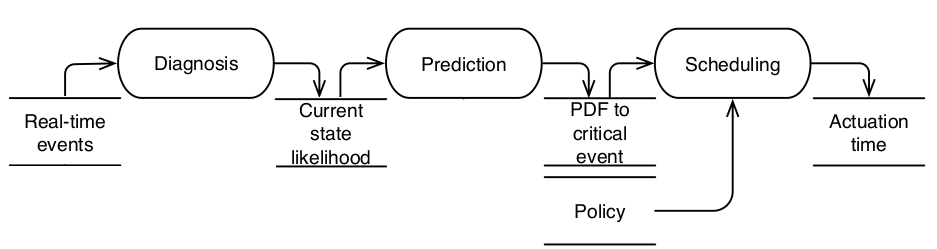
\includegraphics[width=\textwidth,height=0.8\textheight,keepaspectratio]{diag_pred_sched_chain_general.png}
      	\end{center}
      	\begin{tikzpicture}[remember picture, overlay]
        	\node [shift={(-12cm,-5.5cm)}]  at (current page.north east)
        	{%
        		\begin{tikzpicture}[remember picture, overlay]
        			\draw[red, thick] (0,0) rectangle (5cm,2.5cm);
        		\end{tikzpicture}
        	};
      	\end{tikzpicture}
      	
      	\pause
      	La \textbf{diagnosis} calcula el estado efectivo mas probable del modelo en el instante corriente a partir de los eventos observados hasta el instante corriente.
      \end{frame}
    
      \begin{frame}{Diagnosis}{Tiempo discreto}
        \pause
        Los \textbf{Modelos Ocultos de Márkov} (Hidden Markov Model, HMM):
        \pause
        \begin{itemize}
          \item modelan a un sistema parcialmente observable sin tener en cuenta el tiempo de permanencia en cada estado;
          \pause
          \item asocian a cada estado efectivo del sistema una distribución discreta sobre los eventos observables;
          \pause
          \item modelan a un sistema donde los estados efectivos evolucionan como una \textit{Cadena de Márkov Tiempo Discreto} (Discrete Time Markov Chain, DTMC).
        \end{itemize}
        
        \pause
        \visible<6->{
          \begin{center}
            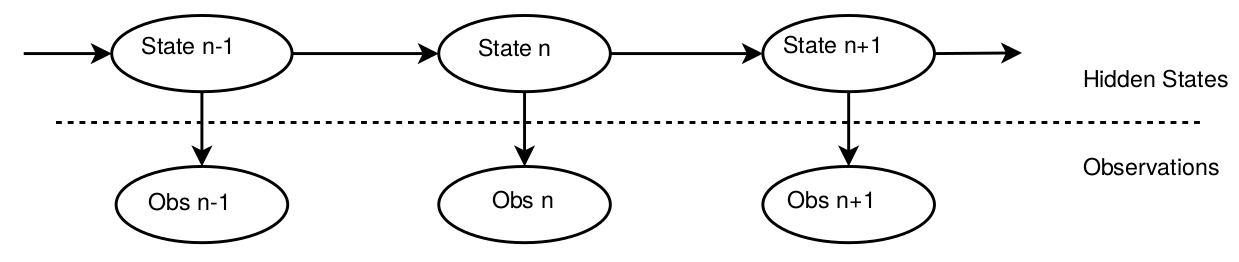
\includegraphics[scale=0.25]{HMM.png}
          \end{center}
        }
        
        \pause
        Diagnosis con HMM se puede lograr con algoritmos clásicos como el \textit{algoritmo de Viterbi} o el \textit{algoritmo de Forward-Backward}.
      \end{frame}
      
      \begin{frame}{Diagnosis}{Tiempo discreto con permanencia}
        \begin{itemize}
          \pause
          \item \textbf{HSMM}\footnote{Van Kasteren, T.L.M., Englebienne, G. and Kröse, B.J., 2010. Activity recognition using semi-markov models on real world smart home datasets. Journal of ambient intelligence and smart environments, 2(3), pp.311-325.}
          \begin{itemize}
            \item Hidden Semi Markov Model;
            \item permanencia en los estados ocultos modelada con distribuciones te tiempo discreto;
            \item eventos generados en cada instante temporal.
          \end{itemize}
          \pause
          \item \textbf{IS-HSMM}/\textbf{ILP-HSMM}\footnote{Narimatsu, H. and Kasai, H., 2016. State Duration and Interval Modeling in Hidden Semi-Markov Model for Sequential Data Analysis. arXiv preprint arXiv:1608.06954.}
          \begin{itemize}
            \item Interval State-Hidden Semi Markov Model;
            \item Interval Length Probability-Hidden Semi Markov Model;
            \item extensiones de los HSMMs;
            \item permite modelar a intervalos de silencio (es decir, sin eventos);
          \end{itemize}
        \end{itemize}
      \end{frame}
      
      \begin{frame}{Diagnosis}{Tiempo continuo}
        \begin{itemize}
          \pause
          \item \textbf{HnMM}\footnote{Buchholz, R., Krull, C., Strigl, T. and Horton, G., 2010, March. Using hidden non-markovian models to reconstruct system behavior in partially-observable systems. In Proceedings of the 3rd International ICST Conference on Simulation Tools and Techniques (p. 86). ICST (Institute for Computer Sciences, Social-Informatics and Telecommunications Engineering).}
          \begin{itemize}
            \item Hidden nonMarkov Model;
            \item tiempos de permanencia continuos;
            \item cada \textit{transición} (es decir, el pasaje de un estado al siguiente) produce un evento.
          \end{itemize}
          \pause
          \item \textbf{GHSMM}\footnote{Salfner, F., 2006. Modeling event-driven time series with generalized hidden semi-Markov models.}
          \begin{itemize}
            \item Generalized Hidden Semi Markov Process;
            \item tiempo de permanencia continuo;
            \item solo una observación por cada estado.
          \end{itemize}
        \end{itemize}
      \end{frame}
      
      \begin{frame}{Diagnosis}{H-MRGP-M}
        \pause
        El \textbf{Modelo Oculto de Márkov Regenerativo} (Hidden-Markov Regenerative Process-Model) ha sido dessarollado por el STLab en la Universidad de Florencia.\footnote{Carnevali, L., Nugent, C., Patara, F. and Vicario, E., 2015, September. A continuous-time model-based approach to activity recognition for ambient assisted living. In International Conference on Quantitative Evaluation of Systems (pp. 38-53). Springer International Publishing.}
        
        \pause
        \begin{itemize}
          \item Modela el tiempo continuo de permanencia en los estados y del inter-tiempo entre eventos.
          \pause
          \item El estado del modelo evoluciona como un \textit{Proceso Regenerativo de Márkov} (Markov Regenerative Process, MRP).
        \end{itemize}
      \end{frame}
      
      \begin{frame}{Diagnosis}{H-MRGP-M: medidas estadísticas}
        \pause
        \begin{itemize}
          \item Experimentado sobre el dataset de van Kasteren:
          \begin{itemize}
            \item 7+1 actividades.
            \item \{Leaving house, Preparing a beverage, Preparing breakfast, Preparing dinner, Sleeping, Taking shower, Toileting\}.
          \end{itemize}
          \pause
          \item A partir de las marcas temporales en el dataset anotado, se calculan medidas estadísticas sobre los tiempos continuos
          \begin{itemize}
            \item de permanencia en cada actividad;
            \item de inter-tiempo entre eventos en cada actividad.
          \end{itemize}
        \end{itemize}
        
        \pause
    		\begin{table}[h!]
    			\centering
    			\small
    			\setlength{\tabcolsep}{5pt}
    			\def\arraystretch{0.75}
    			\begin{tabular}{| l | c | c || c | c |}
    				\hline
    				& \multicolumn{2}{|c||}{\bf Tiempo de permanencia}& \multicolumn{2}{|c|}{\bf Inter-tiempo entre eventos}\\
    				\cline{2-5}
    				& $\mu$ (s) & {\bf CV} & $\mu$ (s) & {\bf CV}\\
    				\hline
    				{\bf Leaving house} & 40\,261.455 & 1.042 & 9\,354.190 & 2.810 \\ \hline
    				{\bf Preparing a beverage} &  35.667 & 1.361 & 7.643 & 2.613\\ \hline
    				{\bf Preparing breakfast} &  108.684 & 0.713 & 9.928 & 1.844\\ \hline
    				{\bf Preparing dinner} &  1\,801.889 & 0.640 & 77.966 & 2.589\\ \hline
    				{\bf Sleeping} &  26\,116.571 & 0.442 & 1\,871.836 & 3.090\\ \hline
    				{\bf Taking shower} &  485.910 & 0.298 & 102.788 & 1.969\\ \hline
    				{\bf Toileting} &  88.742 & 1.175 & 14.814 & 2.449\\ 
    				\hline
      		\end{tabular}
    		\end{table}
      \end{frame}
      
      \begin{frame}{Diagnosis}{H-MRGP-M: modelo estocástico @runtime}
        \pause
        \begin{itemize}
          \item El modelo se crea con técnicas de \textit{process mining}:
          \pause
          \begin{itemize}
            \item \textit{process elicitation} para definir la topología del modelo;
            \pause
            \item \textit{process enhancement} para añadir parámetros estocásticos a partir de las medidas estadísticas calculadas (técnica de Whitt\footnote{Whitt, W., 1982. Approximating a point process by a renewal process, I: Two basic methods. Operations Research, 30(1), pp.125-147.} y software PhFit\footnote{Horváth, A. and Telek, M., 2002, April. Phfit: A general phase-type fitting tool. In International Conference on Modelling Techniques and Tools for Computer Performance Evaluation (pp. 82-91). Springer Berlin Heidelberg.}).
          \end{itemize}
          \pause
          \item Modelo \textbf{@runtime}: modelo actualizado cada vez que se observa un nuevo evento.\footnote{Blair, G., Bencomo, N. and France, R.B., 2009. Models@ run. time. Computer, 42(10).}
          \pause
          \item El formalismo utilizado para representar al modelo es el de las \textbf{Redes de Petri Temporizadas estocásticas} (stochastic Timed Petri Net, sTPN).\footnote{Horváth, A. and Vicario, E., 2009, September. Aggregated stochastic state classes in quantitative evaluation of non-markovian stochastic Petri nets. In Quantitative Evaluation of Systems, 2009. QEST'09. Sixth International Conference on the (pp. 155-164). IEEE.}\footnote{Vicario, E., 2001. Static analysis and dynamic steering of time-dependent systems. IEEE transactions on software engineering, 27(8), pp.728-748.}
        \end{itemize}
      \end{frame}
      
      \begin{frame}{Diagnosis}{H-MRGP-M: sTPN}
        \begin{center}
          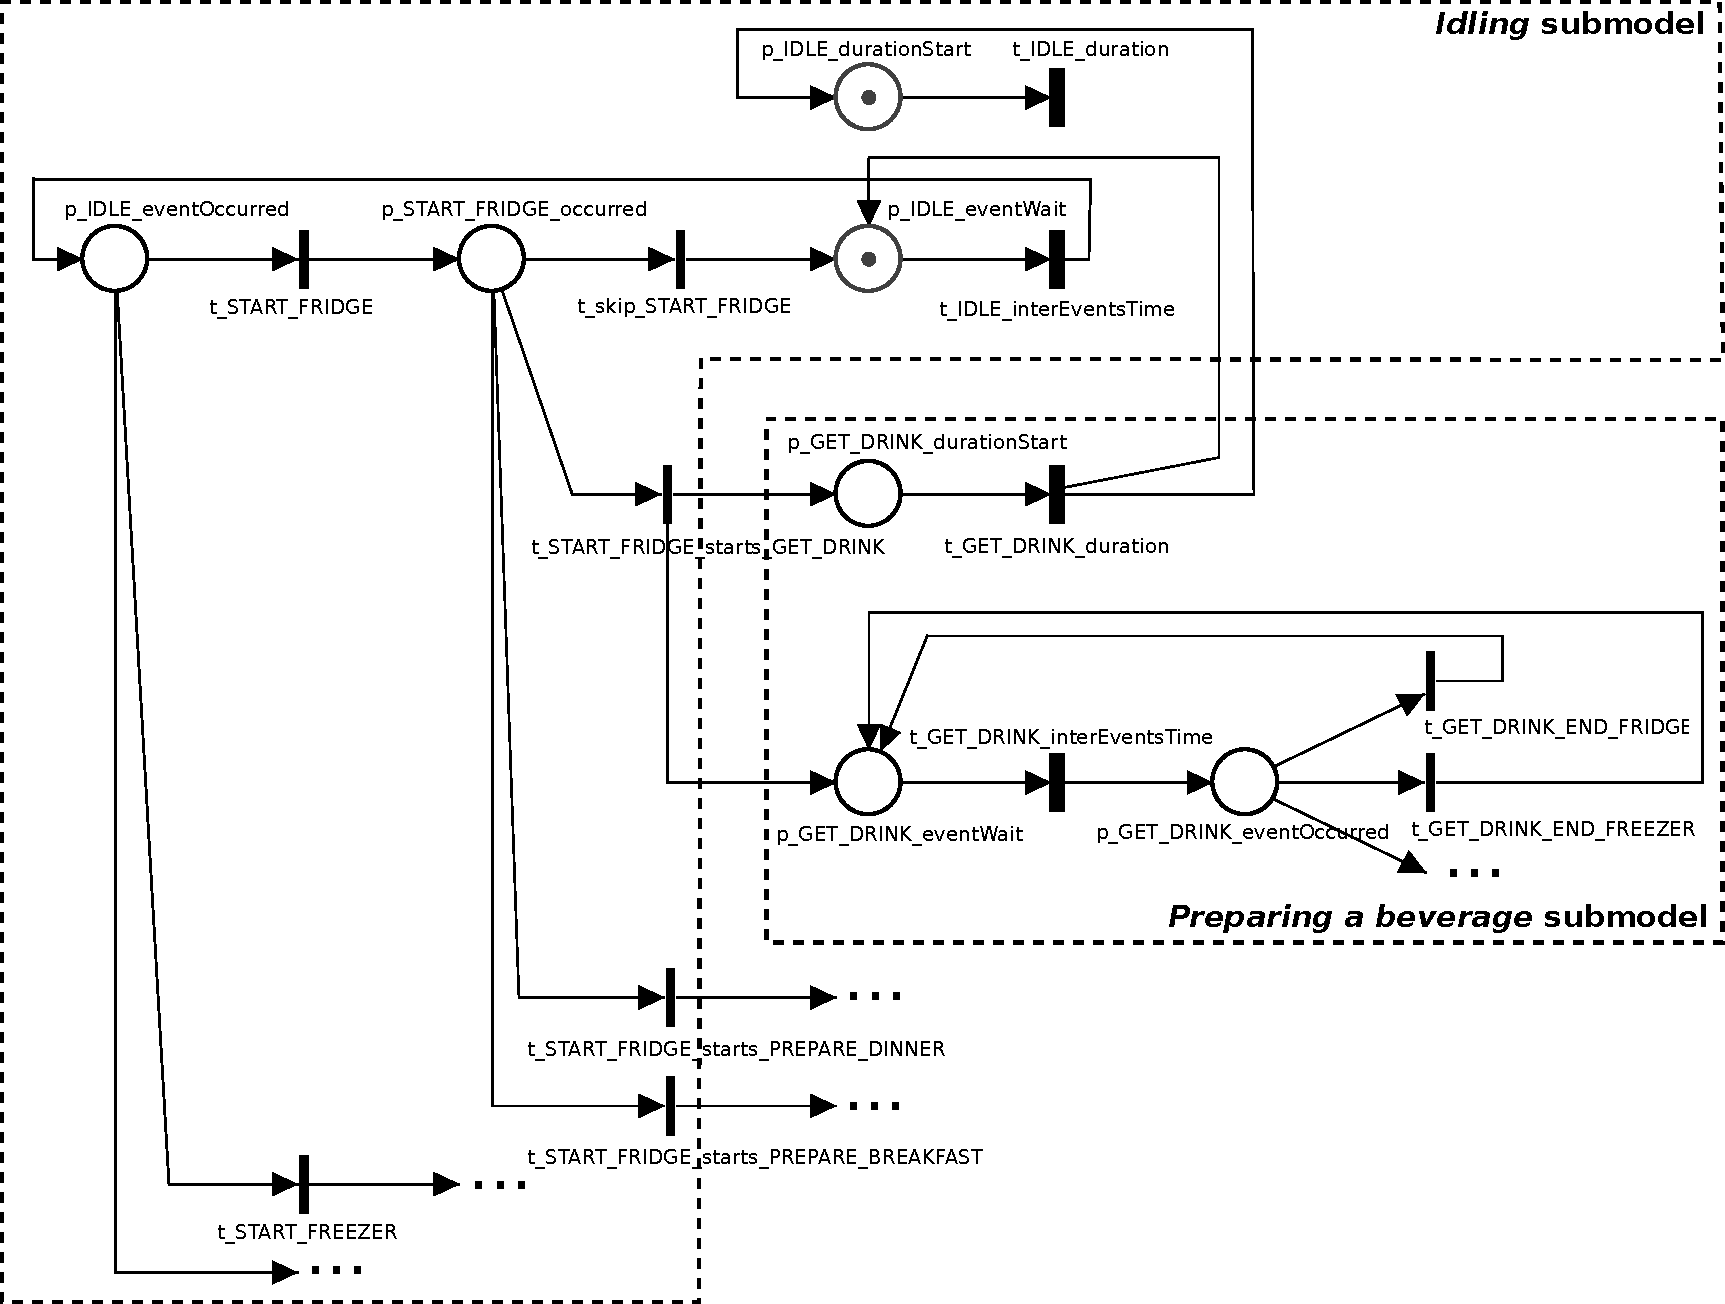
\includegraphics[scale=0.32]{model_withGEN.pdf}
        \end{center}
      \end{frame}
      
      \begin{frame}{Diagnosis}{H-MRGP-M: análisis transitorio}
        \pause
        Después de cada observación, se pueden calcular las probabilidades de estar en diferentes estados del sistema hasta la observación siguiente.
        \pause
        \begin{itemize}
          \item Se explota a la técnica de análisis transitorio de Procesos Regenerativos de Markov basada en clases de estado estocásticas.\footnote{Horváth, A., Paolieri, M., Ridi, L. and Vicario, E., 2012. Transient analysis of non-Markovian models using stochastic state classes. Performance Evaluation, 69(7), pp.315-335.}
        \end{itemize}
        
        \pause
        \visible<4->{
          \begin{center}
            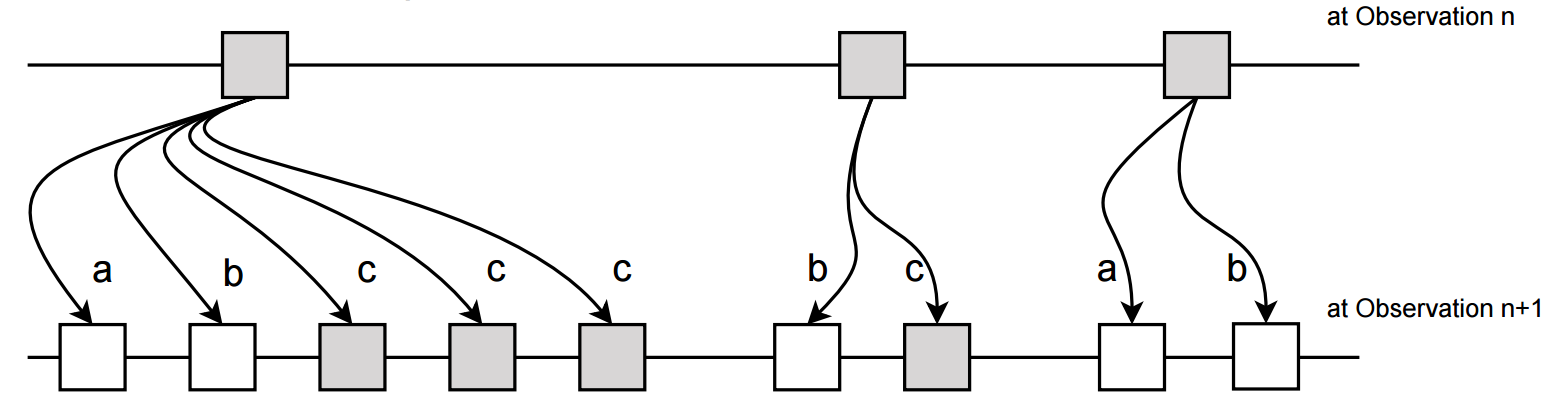
\includegraphics[scale=0.18]{diagnosis-analysis-scheme.png}
          \end{center}
        }
        
        \pause
        El estado estimado por la diagnosis será el estado que lleva la probabilidad más alta.
      \end{frame}
      
      \begin{frame}{Diagnosis}{H-MRGP-M: análisis transitorio}
        \begin{center}
          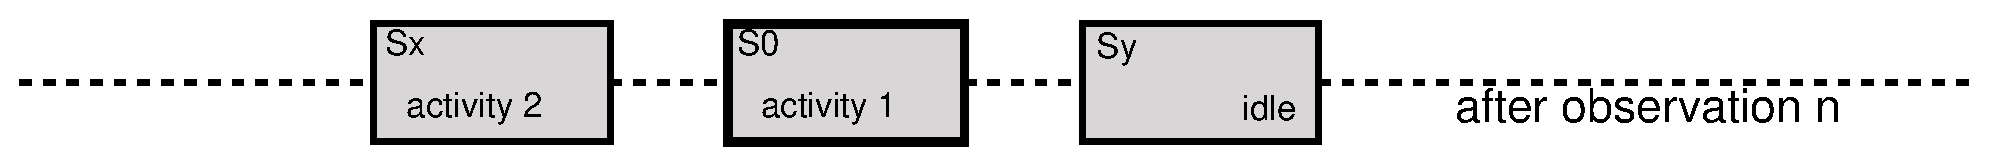
\includegraphics[scale=0.33]{onLineAnalysisAfterN_start.eps}
        \end{center}
        
        \pause
        Después de haber observado el evento $n$, por cada actividad corriente \textit{posible}
        \pause
        \begin{itemize}
          \item se construye el árbol de las clases hasta que se encuentre la observación siguiente (evento $n+1$);
          \pause
          \item se seleccionan las hojas correspondientes al nuevo evento observado;
          \pause
          \item se calcula la PDF de las hojas seleccionadas en el retraso $d$ (inter-tiempo entre los eventos $n$ y $n+1$) en cada árbol, sumandolas entre sí con peso la probabilidad de la raíz;
          \pause
          \item se restituye el máximo como actividad más probable.
        \end{itemize}
      \end{frame}
      
      \begin{frame}{Diagnosis}{H-MRGP-M: análisis transitorio}
        \begin{center}
          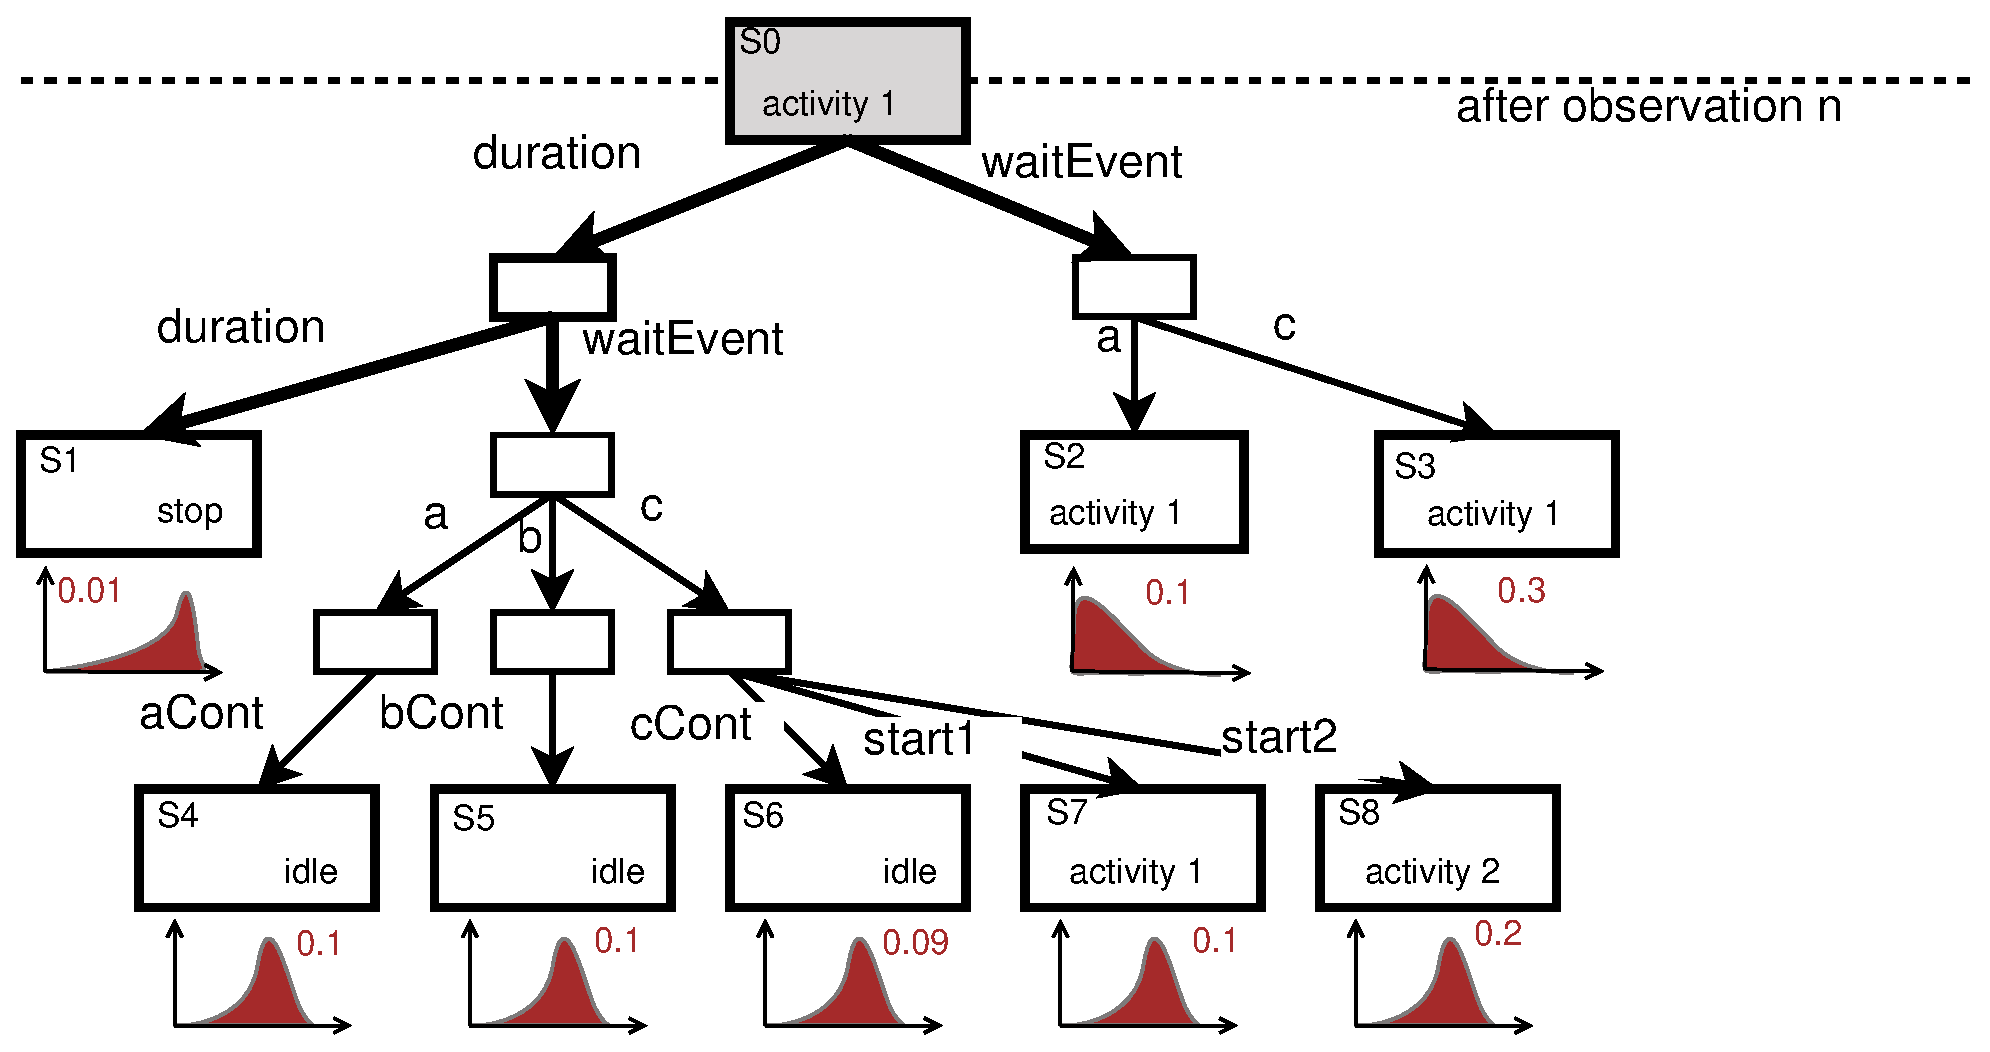
\includegraphics[scale=0.35]{onLineAnalysisAfterN.eps}
        \end{center}
      \end{frame}
      
      \begin{frame}{Diagnosis}{H-MRGP-M: análisis transitorio}
        \begin{center}
          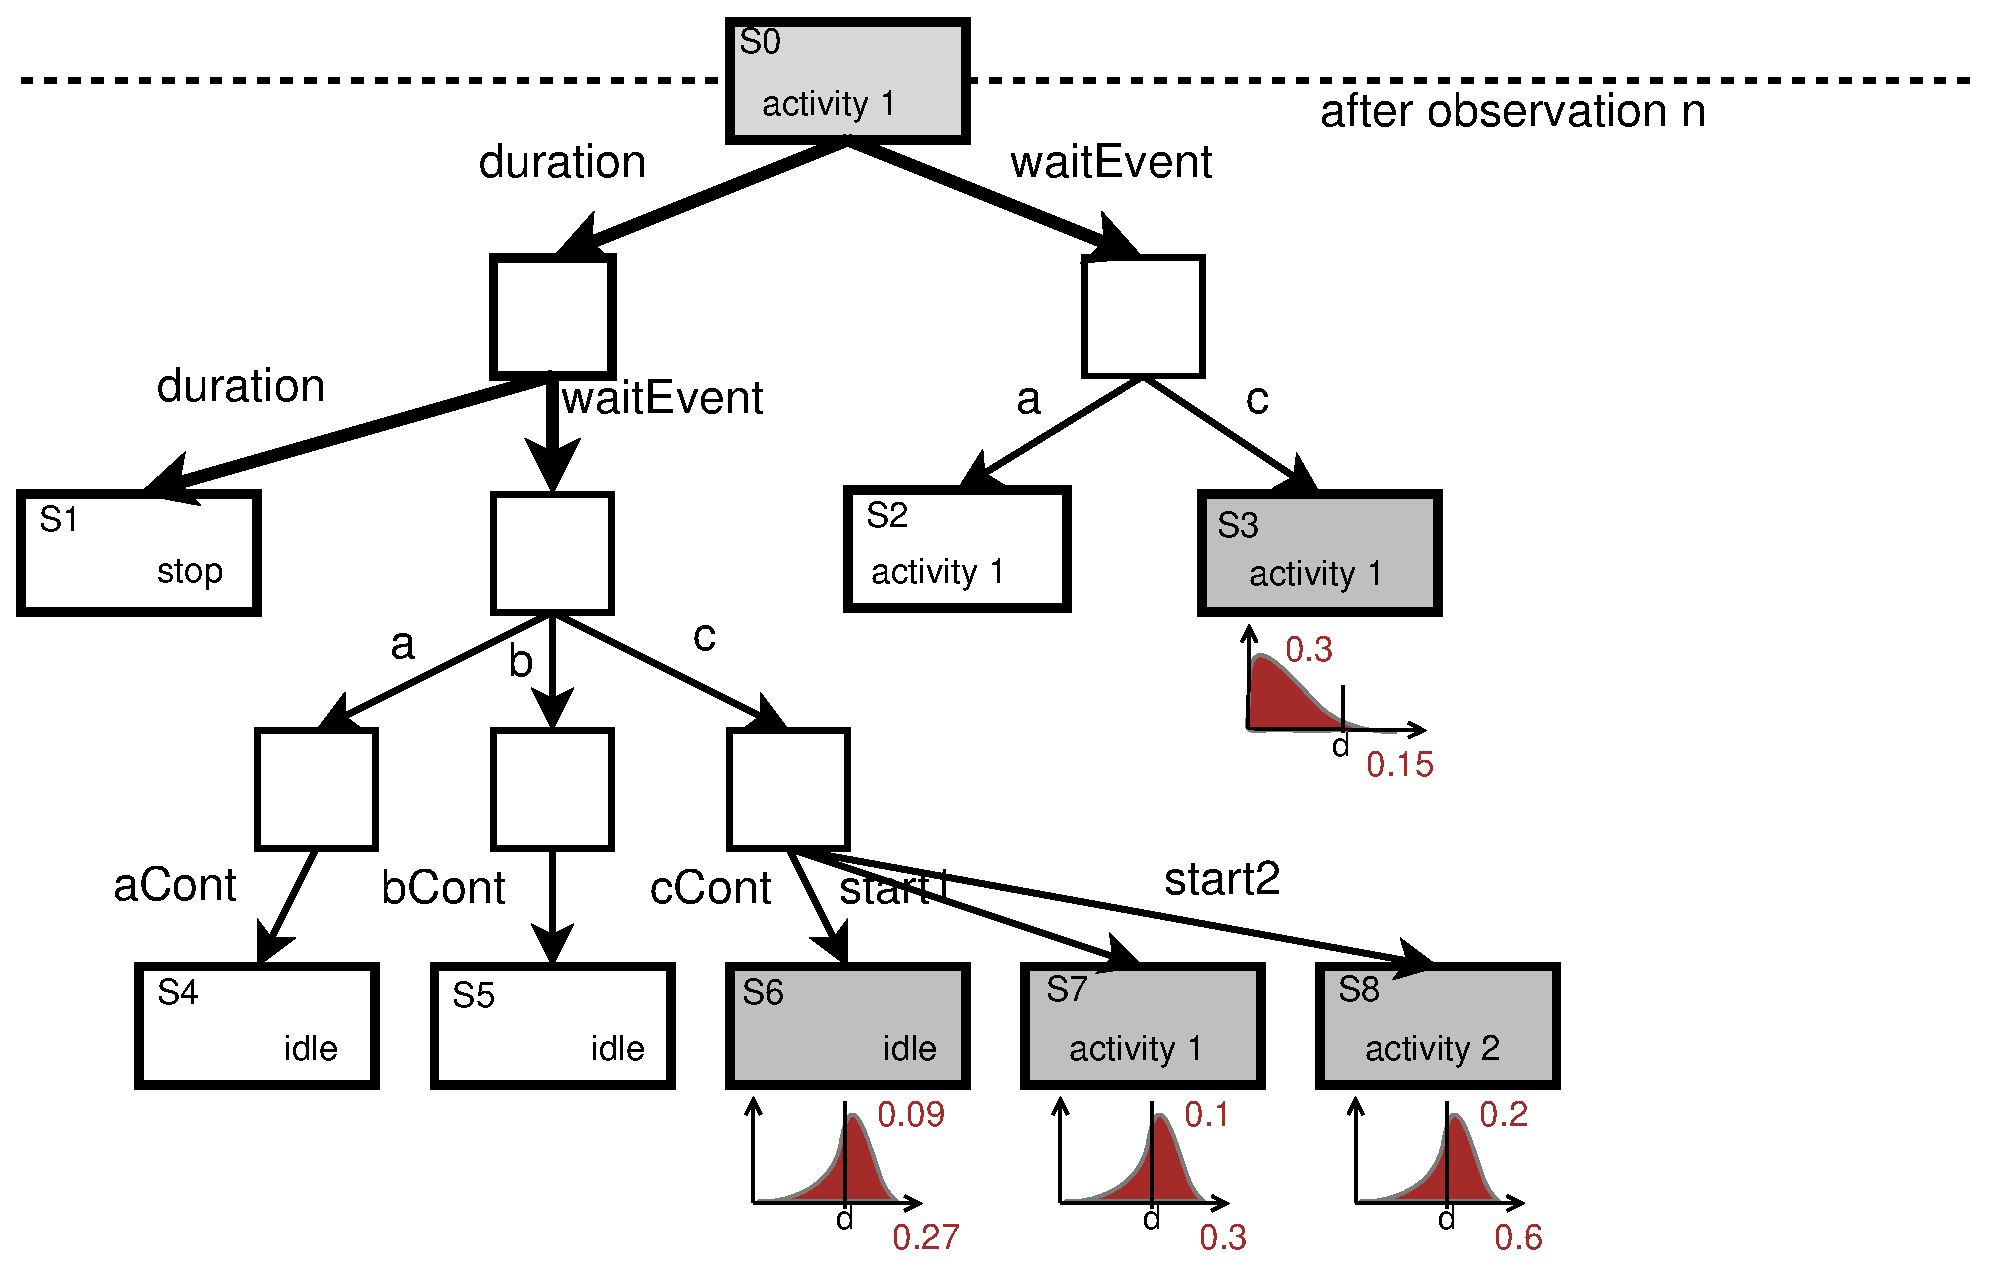
\includegraphics[scale=0.325]{onLineAnalysisAfterN_restricted.eps}
        \end{center}
      \end{frame}
      
    \subsection{Predicción}
      \begin{frame}{Predicción}
      	\begin{center}		
      		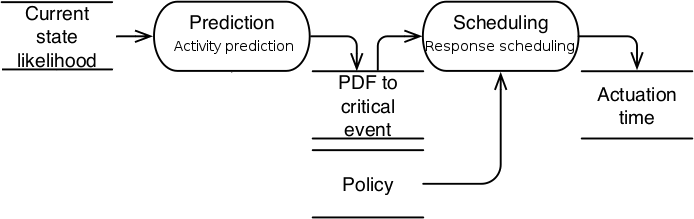
\includegraphics[height=2.8cm,keepaspectratio]{pred_sched_chain.png}
      	\end{center}
      	\begin{tikzpicture}[remember picture, overlay]
        	\node [shift={(-11cm,-4.9cm)}]  at (current page.north east)
        	{%
        		\begin{tikzpicture}[remember picture, overlay]
        		\draw[red, thick] (0,0) rectangle (5.5cm,2.2cm);
        		\end{tikzpicture}
        	};
      	\end{tikzpicture}
      	
      	\pause
      	La \textbf{predicción}\footnote{Salfner, F., Lenk, M. and Malek, M., 2010. A survey of online failure prediction methods. ACM Computing Surveys (CSUR), 42(3), p.10.} calcula la densidad de probabilidad en el tiempo de que ocurra una determinada actividad crítica, a partir de la estimación sobre el estado corriente del modelo calculado por la diagnosis.
      \end{frame}
      
      \begin{frame}{Predicción}{Modelo utilizado}
        \pause
        Predicción de la densidad de probabilidad de una actividad crítica:
        \pause
        \begin{itemize}
          \item Process enhancement sin elicitation:
          \begin{itemize}
            \item probabilidades de transición calculadas por las medidas estadísticas sobre las marcas temporales.
          \end{itemize}
          \pause
          \item Estados \textit{idle} especializados:
          \begin{itemize}
            \item permite tener en cuenta la última actividad.
          \end{itemize}
          \pause
          \item Las actividades evolucionan como un \textit{Proceso Semi Márkov} (Semi Markov Process, SMP).
        \end{itemize}
        
        \pause
        \visible<6->{
        	\begin{figure}[center]
        		\scalebox{0.7}{% -*- TeX:EN:UNIX; ispell-local-dictionary: "american"; TeX-master: "palomar.tex"; -*-
  \scalebox{0.85}{
    \begin{tikzpicture}[label distance=1mm,>=stealth',auto,font=\sffamily,font=\small,node distance=15mm and 5mm,/tikz/initial text=]
    \tikzstyle{state-act}=[circle,rounded corners,draw,fill=gray!30,text height=1.7ex,text depth=0.3ex,anchor=base,text centered,text width=9mm, minimum height=9mm]
    \tikzstyle{state-idle}=[circle,rounded corners,draw,fill=black!0,text height=1.7ex,text depth=0.3ex,anchor=base,text centered,text width=9mm, minimum height=9mm]

    \node [state-act,initial] (x) at (0,6.07cm) { $\texttt{act}_x$};
    \node [state-act] (y) at (9cm,6.07cm) { $\texttt{act}_y$};
    \node [state-act] (z) at (4.5cm,4cm) { $\texttt{act}_z$};
    \node [state-idle] (xz) at (1cm,4cm) {$\texttt{idle}_{xz}$};
    \node [state-idle] (yz) at (8cm,4cm) {$\texttt{idle}_{yz}$};
    \node [state-idle] (xy) at (4.5cm,7.7cm) {$\texttt{idle}_{xy}$};
    \node [state-idle] (yx) at (4.5cm,6.07cm) {$\texttt{idle}_{yx}$};
    \path (z.base) -- node[midway,state-idle] (zx) {$\texttt{idle}_{zx}$} (x.base);
    \path (z.base) -- node[midway,state-idle] (zy) {$\texttt{idle}_{zy}$} (y.base);
    \draw[->] (x) to node[] {$p_{xy}$} (xy);
    \draw[->] (xy) to (y);
    \draw[->] (y) to node[above] {$p_{yx}$} (yx);
    \draw[->] (yx) to (x);
    \draw[->] (x) to node[left] {$p_{xz}$} (xz);
    \draw[->] (xz) to (z);
    \draw[->] (z) to node[above] {$p_{zx}$} (zx);
    \draw[->] (zx) to (x);
    \draw[->] (y) to node[right] {$p_{yz}$} (yz);
    \draw[->] (yz) to (z);
    \draw[->] (z) to node[above] {$p_{zy}$} (zy);
    \draw[->] (zy) to (y);
   %  \node [class, right=of s2,xshift=1.5cm] (s5) {
   %    $S_5|$ $\id{buffer_1}\,\id{producing_2}$\\
   %    $(\id{consume_1},\id{produce_2}) \in [1,2]\times [0,2]$
   %  };
   % 
   % \draw[->] (s0) to  node[left] {$\tr{produce_2}$} (s0 |- s9.south);
  \end{tikzpicture}
  }
}
        	\end{figure}
        }
      \end{frame}
      
      \begin{frame}{Predicción}{Calculo de la PDF}
        \pause
        \vspace{-1em}
      	\visible<2->{
        	\begin{center}
	\scalebox{0.78}{\begin{tikzpicture}
	    \tikzstyle{state}=[circle,rounded corners,draw,fill=black!0,text height=1.7ex,text depth=0.3ex,anchor=base,text centered,text width=5mm, minimum height=5mm]
		\def\innercirclesize{4mm} 
	
		\node [state] (stateA) at (0, 2cm) { $A$};
		\draw[thick,dashed] (0, 2.13cm) circle (\innercirclesize);
		\node [state] (stateB) at (0, 0) { $B$};
		\draw[thick,dashed] (0, 0.13cm) circle (\innercirclesize);
		\node [state] (stateC) at (2cm, 0.5cm) { $C$};
		\node [state] (stateD) at (2cm, 2.5cm) { $D$};
		\node [state] (stateE) at (4cm, 2.5cm) {$E$};
		\node [state,fill=gray] (stateF) at (4cm, 0.5cm) { $F$};
	
	
		\draw[->] (stateA) to (stateC);
		\draw[->] (stateA) to (stateD);
		\draw[->] (stateB) to (stateC);
		\draw[->] (stateC) to (stateF);
		\draw[->] (stateD) to (stateC);
		\draw[->] (stateD) to (stateF);
		\draw[->] (stateF) to (stateE);
		\draw[->] (stateE) to (stateD);
		
		\node [above=-0.15cm of stateA] {$\pi_A = 0.7$};
		\node [above=-0.15cm of stateB] {$\pi_B = 0.3$};
	
	\end{tikzpicture}}
\end{center}
        }
        
      	\pause
      	\begin{itemize}
        	\item Para cada estado posible, se calcula la densidad de probabilidad de alcanzar al estado crítico (análisis transitorio).
        	\pause
        	\item Se suman entre sí las densidades de probabilidad a partir de cada estado posible, pesadas por la probabilidad de estar en cada estado.
      	\end{itemize}
      	
      	\pause
      	\vspace{-1em}
      	\visible<5->{
        	\begin{tikzpicture}[scale=1]
%Plot A
\node[inner sep=0pt] at (0,0)
{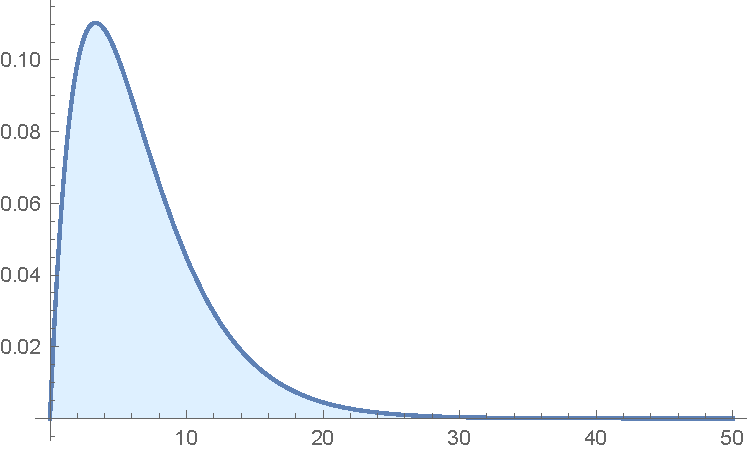
\includegraphics[width=.30\textwidth]{plot1.pdf}};
\node at(-0.7,1.5) {$PDF(t)_{A\_to\_F} * \pi_{A}$};
\node at(1.9,-0.9) {$t$};

%Plot B
\node[inner sep=0pt] at (4,0)
{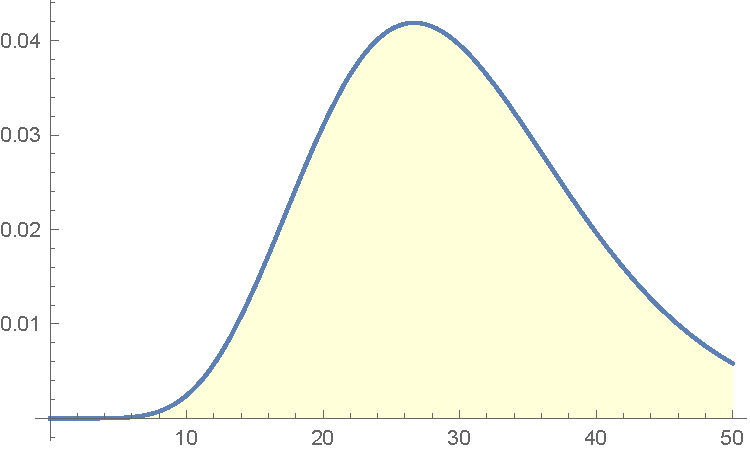
\includegraphics[width=.30\textwidth]{plot2.pdf}};
\node at(3.3,1.5) {$PDF(t)_{B\_to\_F} * \pi_{B}$};
\node at(5.9,-0.9) {$t$};

%Sum of plots
\node[inner sep=0pt] at (8,0)
{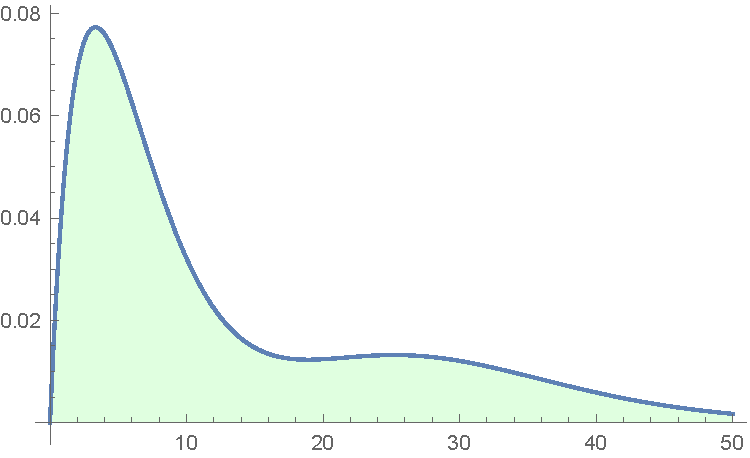
\includegraphics[width=.30\textwidth]{sumPlot.pdf}};
\node at(7.2,1.5) {$PDF(t)_{to\_F}$};
\node at(9.9,-0.9) {$t$};

%operation simbol
\draw[fill=white] (1.7,0.30) circle [radius=0.3] node {+};
\draw[fill=white] (5.7,0.30) circle [radius=0.3] node {=};
	
\end{tikzpicture}

        }
      \end{frame}
      
    \subsection{Planificación de acciones}
      \begin{frame}{Planificación de acciones}
      	\begin{center}		
      		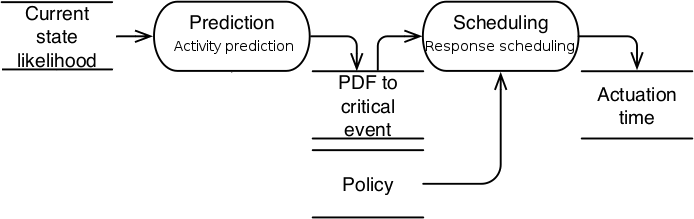
\includegraphics[height=2.8cm,keepaspectratio]{pred_sched_chain.png}
      	\end{center}
      	\begin{tikzpicture}[remember picture, overlay]
        	\node [shift={(-6.9cm,-6.1cm)}]  at (current page.north east)
        	{%
        		\begin{tikzpicture}[remember picture, overlay]
        		\draw[red, thick] (0,0) rectangle (5.3cm,3.2cm);
        		\end{tikzpicture}
        	};
      	\end{tikzpicture}
      	
      	\pause
      	La \textbf{planificación de acciones} calcula el instante temporal óptimo para planificar una reacción oportuna a una determinada actividad critica, a partir de la probabilidad de que dicha actividad ocurra (calculada por la predicción) y de una política de reacción (decidida por el usuario).
      \end{frame}
    
      \begin{frame}{Planificación de acciones}{Descripción del problema\footnote{Biagi, M., Carnevali, L., Paolieri, M., Patara, F. and Vicario, E., 2016, October. A Stochastic Model-Based Approach to Online Event Prediction and Response Scheduling. In European Workshop on Performance Engineering (pp. 32-47). Springer International Publishing.}}
        \pause
        \begin{itemize}
          \item \textbf{Actividad crítica}: actividad por la cual nos interesa planificar una reacción.
          \pause
          \item \textbf{Reacción}: acción que el sistema tiene que actuar cuando ocurre la actividad crítica.
          \pause
          \item \textbf{Duración de la reacción}: duración $t_d$ del tiempo de activación de la reacción.
          \pause
          \item \textbf{Tiempo de actuación de la reacción}: tiempo $t_w$ necesario al sistema para llevar a cabo la reacción desde cuando ha sido planificada.
        \end{itemize}
        
        \pause
       	\begin{columns}
       		\column{0.60\linewidth}
       		\centering
       		\tikzset{>=stealth'}
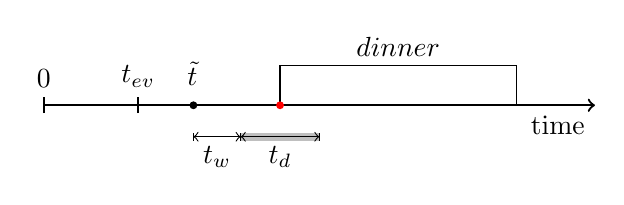
\begin{tikzpicture}[scale=1]
  \tikzset{
    activity/.style={dashed}
    schedule/.style={dashed, color=black!5}
  }
  \def\tickheight{2mm}
  \def\eticka{1.2}
  \def\etickb{2.2}
  \def\etickc{4.2}
  \def\etickd{7}
  \def\eticke{8}
  \def\actheight{0.5cm}
  \def\astarta{.5}
  \def\aenda{3.2}
  \def\astartb{6}
  \def\aendb{9}
  \def\D{1}
  \def\W{.6}
  \def\shiftpdfc{-0.4cm}
  \def\startpredc{1.3}

  
  \draw[->,thick] (3,0) --  (10,0) node[below left] {time};
  \draw[thick] (3,-{\tickheight/2}) -- (3,{\tickheight/2}) node[above] {0};
  
  \draw[thick] (\etickc,-{\tickheight/2}) node[below] {} -- (\etickc,{\tickheight/2}) node[above] {$t_{ev}$} ;
  
%  \draw[thick] (\astartb,-{\tickheight/2}) node[below] {$\tau_2$} -- (\astartb,{\tickheight/2}) ;
%  \draw[thick] (\aendb,-{\tickheight/2}) node[below] {$\tau_2+\delta_2$} -- (\aendb,{\tickheight/2}) ;
  \draw[activity] (\astartb,0) -- (\astartb,\actheight) -- node[above] {$dinner$} (\aendb,\actheight) -- (\aendb,0);
  \fill[red] (\astartb,0) circle (.5mm);

  \begin{scope}[xshift=\etickc cm, yshift=\shiftpdfc]


    \draw [line width=1mm,color=black!25]({\startpredc},0) -- ({\startpredc+\D},0);
    \draw (\startpredc,-{\tickheight/4}) -- (\startpredc,{\tickheight/4});
    \draw ({\startpredc+\D},-{\tickheight/4}) -- ({\startpredc+\D},{\tickheight/4});
    \draw [<->]({\startpredc},0) -- ({\startpredc+\D},0);
    \node[below] at ({\startpredc+\D/2},0) {$t_d$};

    \draw (\startpredc,-{\tickheight/4}) -- (\startpredc,{\tickheight/4});
    \draw ({\startpredc-\W},-{\tickheight/4}) -- ({\startpredc-\W},{\tickheight/4});
    \draw [<->]({\startpredc},0) -- ({\startpredc-\W},0);
    \node[below] at ({\startpredc-\W/2},0) {$t_w$};


    \node [right] at ({\startpredc-(.8)},0.8cm) {$\tilde t$};
    
    
  \end{scope}
  \fill[black] ({\startpredc-\W+\etickc},0) circle (.5mm);
\end{tikzpicture}

       		\column{0.40\linewidth}
       		Por ej. notificación para tomar pastillas antes de cenar:
       		\begin{itemize}
       			\item $t_w = 60s$
       			\item $t_d = 120s$
       			\item Notifica al instante $\tilde t$
       		\end{itemize}
       	\end{columns}
      \end{frame}
      
      \begin{frame}{Planificación de acciones}{Politica de planificación}
        \pause
        \begin{itemize}
          \item Se busca el \textbf{intervalo de mayor probabilidad} (de longitud $t_d$) de que ocurra la actividad crítica.
          \pause
          \item Si la \textbf{probabilidad máxima} está mas alta de un \textbf{umbral fijo}, la reacción será planificada por el sistema al instante $\boldsymbol{\tilde t = x^* - t_w}$, donde $x^*$ indica el extremo inferior del intervalo de máxima probabilidad.
          \pause
          \item Si la probabilidad máxima está mas baja del umbral, ninguna reacción será planificada por el sistema.
        \end{itemize}
        
        \pause
        \vspace{-1em}
        \centering
        \tikzset{>=stealth'}
\begin{tikzpicture}[scale=1]
  \tikzset{
    activity/.style={dashed}
    schedule/.style={dashed, color=black!5}
  }
  \def\tickheight{2mm}
  \def\eticka{1.2}
  \def\etickb{2.2}
  \def\etickc{4.2}
  \def\etickd{7}
  \def\eticke{8}
  \def\actheight{0.5cm}
  \def\astarta{.5}
  \def\aenda{3.2}
  \def\astartb{6}
  \def\aendb{9}
  \def\D{1}
  \def\W{.6}
  \def\shiftpdfc{-1.6cm}
  \def\startpredc{1.3}

  
  \draw[->,thick] (3,0) --  (10,0) node[below left] {time};
  \draw[thick] (3,-{\tickheight/2}) -- (3,{\tickheight/2}) node[above] {0};
  
  \draw[thick] (\etickc,-{\tickheight/2}) node[below] {} -- (\etickc,{\tickheight/2}) node[above] {$t_{ev}$} ;
  
%  \draw[thick] (\astartb,-{\tickheight/2}) node[below] {$\tau_2$} -- (\astartb,{\tickheight/2}) ;
%  \draw[thick] (\aendb,-{\tickheight/2}) node[below] {$\tau_2+\delta_2$} -- (\aendb,{\tickheight/2}) ;
  \draw[activity] (\astartb,0) -- (\astartb,\actheight) -- node[above] {$dinner$} (\aendb,\actheight) -- (\aendb,0);
  \fill[red] (\astartb,0) circle (.5mm);

  \begin{scope}[xshift=\etickc cm, yshift=\shiftpdfc]
    \begin{scope}[on background layer]
    \draw[color=black!30,dashed] ({\startpredc-\W},1mm) -- ({\startpredc-\W},-\shiftpdfc);
    \draw[color=black!15] ({\astartb-\etickc},.5mm) -- ({\astartb-\etickc},-\shiftpdfc);
    \end{scope}
    \draw[<->] (0,1cm) node[below left] {$PDF(t)$} -- (0,0) --  (4cm,0) node[right] {$t$};

    \draw [line width=1mm,color=black!25]({\startpredc},0) -- ({\startpredc+\D},0);
    \draw (\startpredc,-{\tickheight/4}) -- (\startpredc,{\tickheight/4});
    \draw ({\startpredc+\D},-{\tickheight/4}) -- ({\startpredc+\D},{\tickheight/4});
    \draw [<->]({\startpredc},0) -- ({\startpredc+\D},0);
    \node[below] at ({\startpredc+\D/2},0) {$t_d$};

    \draw (\startpredc,-{\tickheight/4}) -- (\startpredc,{\tickheight/4});
    \draw ({\startpredc-\W},-{\tickheight/4}) -- ({\startpredc-\W},{\tickheight/4});
    \draw [<->]({\startpredc},0) -- ({\startpredc-\W},0);
    \node[below] at ({\startpredc-\W/2},0) {$t_w$};

    \draw [red] plot [smooth] coordinates {(0,0) (1,.5) (1.8,1) (2.5,.6) (3.5,0.2) (3.8,0)};
    \node [right] at ({\startpredc-(.8)},2.0cm) {$\tilde t$};
    
    \node [above] at ({\startpredc+0.1},0) {$x^*$};
    
  \end{scope}
  \fill[black] ({\startpredc-\W+\etickc},0) circle (.5mm);
\end{tikzpicture}

      \end{frame}
      
  \section*{Fin}
    \begin{frame}
      \begin{center}
      	\textbf{\calligra\Huge Fin.}\\
        
\includegraphics[width=5cm]{ornament.eps}
        
      	\pause
      	\vspace{1cm}
      	{\huge\calligra Preguntas?\pause{} Gracias!}
      \end{center}
    \end{frame}
      
\end{document}
